\iffalse

\chapter{Fundamentarea teoretică și documentarea bibliografică}
\label{cap:cap1}

(10–15 pagini)\footnote{Template-ul a fost construit similar celui dezvoltat de George VIERIU, disponibil la \url{https://ac.tuiasi.ro/studenti/didactic/finalizare-studii/finalizare-studii-calculatoare/finalizare-studii-calculatoare-ghidul-studentului/}}

\begin{itemize}
    \item Domeniul și contextul abordării temei;
    \item Tema propusă (formularea exactă a temei, obiective, justificarea abordării);
    \item Prezentare succintă și comparativă privind realizările actuale pe aceeași temă;
    \item Analiza tipurilor de produse/aplicații existente din respectiva categorie a temei,
tehnologii folosite pentru implementare;
    \item Elaborarea specificațiilor privind caracteristicile așteptate de la aplicație. 
\end{itemize}

Lucrările utilizate în dezvoltarea proiectului de diplomă și în redactarea tezei vor fi citate corespunzător în cadrul prezentului document. Această citare trebuie să fie o interpretare sau o descriere proprie autorului prezentei teze asupra ideii/soluției/conceptului prezentat în lucrarea sursă și \textbf{\textit{nu}} o preluare mot-a-mot sau o traducere directă. O posibilă excepție de la această regulă se poate face în cazul rezultatelor teoretice importante, cum ar fi, de exemplu, definițiile, teoremele sau algoritmii suport. În textul asociat citării este recomandat să includeți, de asemenea, și o frază prin care să realizați legătura cu lucrarea proprie. Teza capătă în acest fel consistență și evitați ideea de citare bulk, „doar ca să fie". În continuare vă prezentăm un scurt exemplu.

\todo[inline]{TO DO: Aici ar trebui să introduc o referință bibliografică deoarece ceea ce am scris nu este ideea mea}

Mironeanu et. al. propun o nouă abordare pentru monitorizarea și prevenția atacurilor cibernetice \cite{art:mironeanu:ECAD:2021}. Soluția utilizează tehnici de tip AI/ML și pe un sistem de votare ponderat cu scopul de determina dacă un acces în rețea este un acces normal sau un eventual atac. Pornind de la noțiunile descrise în \cite{art:mironeanu:ECAD:2021}, lucrarea de față își propune îmbunătățirea detecției atacurilor de tip \textit{flood}.

Pornind de la modelul REST propus de Fielding în \cite{thesis:fielding:2000} și considerând specificațiile protocolului HTTP \cite{misc:web:rfc7231}, Archip et. al. demonstrează în \cite{inproc:archip:restful:2018} faptul că o utilizare greșită a modelului amintit poate conduce la o slăbire a securității unui server. Un alt aspect important care trebuie considerat cu privire la securitatea sistemelor informatice este legat de utilizatori. Acest subiect este tratat pe larg în \cite{incollection:ARASEC2020}.

Un exemplu de intrare bibliografică pentru un \textit{tech report} este în \cite[p.~13]{IEEEexample:techreptypeii} (numărul paginii este trecut explicit în sursă). Bineînțeles, nu putem discuta despre configurările și instalările unor sisteme Cloud Computing \cite[p.~113]{book:marinescu:2018}, dacă nu considerăm și sistemele de operare suport sau gazdă \cite{book:operating_systems:2014}. În cazul în care dorim să referim o pagină web care nu se încadrează în categoriile carte, articol, raport tehnic, putem să utilizăm o intrare de tip \verb|misc| în bibliografie. Recomandarea este să utilizăm documente Web publicate de companii importante (precum IBM, RedHat, Apple, etc.) sau personalități recunoscute, precum Bruce Schneier \cite{misc:web:schneier2021}.

\textcolor{gray}{\lipsum}(Figura \ref{fig:puterea_furnizata_pe_cm_cub})

\begin{figure}[H]
    \centering
    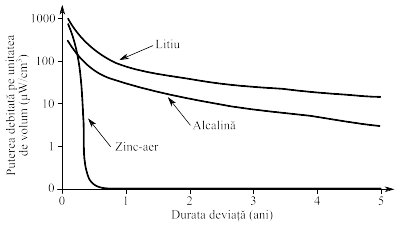
\includegraphics[width=0.6\textwidth]{continut/capitol1/figuri/puterea_furnizata_pe_cm_cub.png}
    \caption{Puterea furnizată pe cm\textsuperscript{3} relativă la durata de viață pentru trei tipuri de baterii.}
    \label{fig:puterea_furnizata_pe_cm_cub}
\end{figure}

\textcolor{gray}{\lipsum}

\section{Exemplu de subcapitol nivel 1}
\label{cap:cap1:ex-subcapitol}

\textcolor{gray}{\lipsum} (Figura \ref{fig:r2_d2})

\begin{figure}[t]
    \centering
    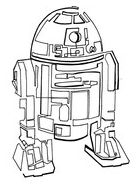
\includegraphics[width=0.25\textwidth]{continut/capitol1/figuri/r2_d2.png}
    \caption{R2-D2\protect\footnotemark}
    \label{fig:r2_d2}
\end{figure}
\footnotetext{imagine preluată de pe un site web care nu „merită” trecut la bibliografie \url{https://www.shutterstock.com/}}

\textcolor{gray}{\lipsum} 

\subsection{Exemplu de subcapitol nivel 2}
\label{cap:cap1:ex-supcapitol:nivel2}

\textcolor{gray}{\lipsum} (Figura \ref{fig:yoda})

\begin{figure}[H]
    \centering
    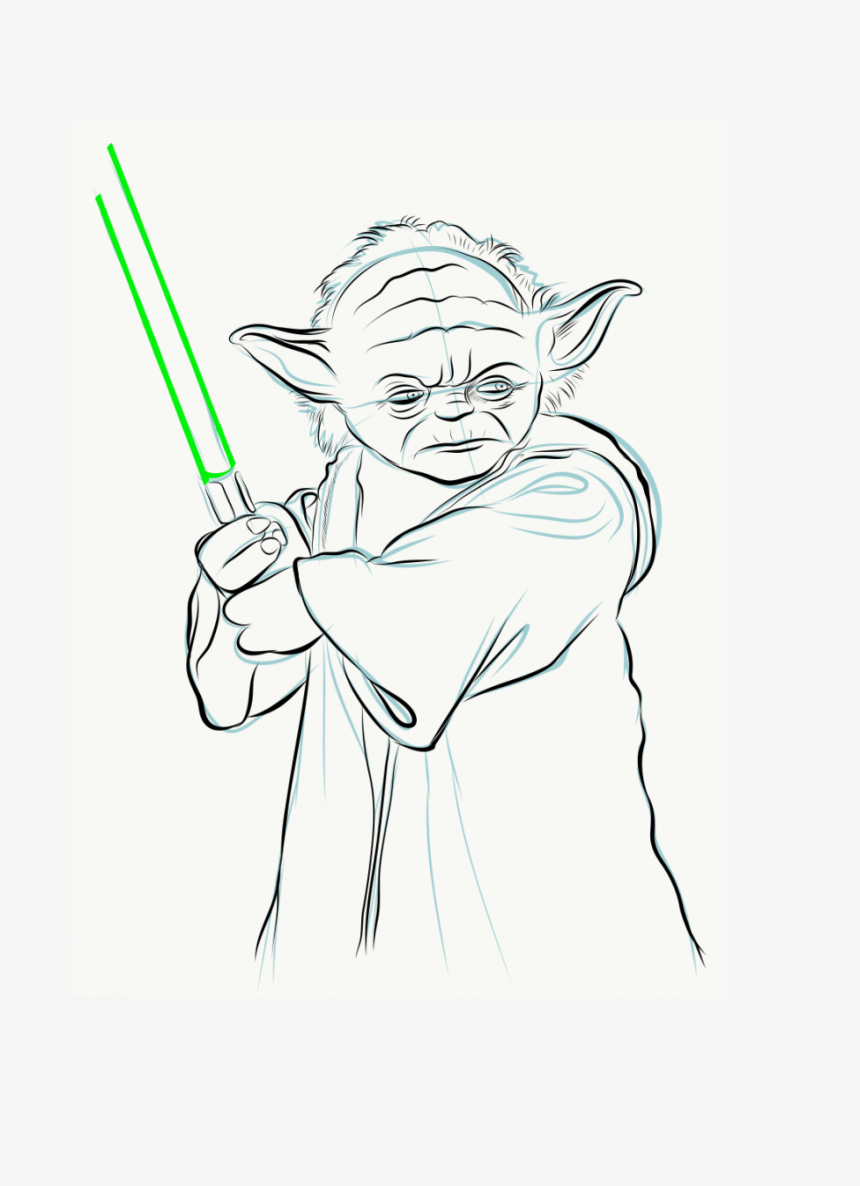
\includegraphics[width=0.3\textwidth]{continut/capitol1/figuri/yoda.png}
    \caption{Yoda\protect\footnotemark}
    \label{fig:yoda}
\end{figure}
\footnotetext{imagine preluată de pe un site web care nu „merită” trecut la bibliografie \url{https://www.pngitem.com/}}

\textcolor{gray}{\lipsum}

\subsubsection{Exemplu de subcapitol nivel 3}
\label{cap:cap1:ex-subcapitol:nivel2:nivel3}

\textcolor{gray}{\lipsum}

Următoarele e fără label FTW, decât să demonstrez gen!\footnote{Dacă vă prindem cu astfel de exprimări, vă scădem 2 puncte!!!}

\section{Nivel 1}
\label{cap:cap1:nivel1}

\subsection{Nivel 2}
\label{cap:cap1:nivel1:nivel2}

Ghilimelele se pun înainte și după reproducerea unui text. Se pun între semnele citării cuvintele sau grupurile de cuvinte citate ironic sau care redau atitudinea rezervată ori dezaprobatoare a autorului față de realitățile pe care le desemnează respectivele cuvinte. Se obișnuiește să se pună între ghilimele titlurile operelor literare de artă sau științifice, ale publicațiilor, numele instituțiilor, firmelor etc. atunci când aceste titluri sunt reproduse într-o frază. 
Atenție: Ghilimelele limbii engleze (“ ”) sunt diferite de ghilimelele limbii române („ ”)!
Observație: Documentele tehnice au adoptat din sintaxa limbajelor de programare ghilimelele duble (") pentru a evidenția șirurile de caractere în text și ghilimelele simple (') pentru evidențierea caracterelor. De exemplu: "acesta este un șir de caractere", acesta este caracterul 'x'.

\subsubsection{Nivel 3}
\label{cap:cap1:nivel1:nivel2:nivel3}

Oricum, mai departe de \verb|#.#.#.#| \textbf{\textit{NU}} trebuie să se ajungă :P.

\fi


\chapter{Fundamentarea teoretică și documentarea bibliografică}
\label{cap:cap1}

Structura următoarelor câteva subcapitole este puternic influențată de structura cursului de Calcul Cuantic din cadrul Facultății de Informatică de la Universitatea "Alexandru Ioan Cuza", predat de doamna Conf. Arusoaie Andreea, fără de care această lucrare probabil că nu ar fi fost posibilă. Voi încerca a prezenta doar elementele relevante, pe scurt, pentru această lucrare, rezumând / scurtând / eliminând acele elemente care nu vor avea nici o legătură cu lucrarea.

\section{Elemente de algebră liniară}

\subsection{Mulțimea numerelor complexe}

Mulțimea numerelor complexe este un sistem de numărare care conține numerele reale și o unitate imaginară $i$ care îndeplinește proprietatea:
\[i^2 = -1\]
Uneori, definiția unității imaginare este dată in literatura de specialitate ca fiind: \[i = \sqrt{-1}\]
Se numește număr complex orice număr de forma \[z = a + ib,\] unde $a$ și $b$ sunt numere reale. Mulțimea numerelor complexe $\mathbb{C}$ este așadar definită în felul următor: 
\[ \mathbb{C} = \{z \enspace|\; z = a + ib,\enspace a,\enspace b \enspace\in\enspace \mathbb{R},\enspace i^2 = -1\} \]

Conjugatul unui număr complex $z$ este definit ca:
\[\bar{z} \overset{not.}{=} z\text{*} = a - ib\]
Notația cu bară deasupra pentru $z$ este deseori utilizată în matematică, iar notația cu asterisc este utilizată mai des în fizică. Pe parcursul acestei lucrări se va folosi a doua notație.

Modulul sau amplitudinea unui număr complex:
\[z = \sqrt{a^2 + b^2}\]

\textbf{Proprietăți ale numerelor complexe}:

Fie $z, w \in \mathbb{C}$. Atunci au loc:
\begin{itemize}
    \item $\overline{z + w} = \bar{z} + \bar{w}$ 
    \item $z \cdot \bar{z} = \bar{z} \cdot z = |z|^2$
    \item $\bar{\bar{z}} = z$
    \item $|z| = |\bar{z}|$
\end{itemize}
\pagebreak

Forma trigonometrică a numerelor complexe este dată de formula:
\[z = A(\cos \theta + i \sin \theta) = Ae^{i\theta}\] 

Unde $A = \sqrt{a^2 + b^2}$,  $\theta = \arctan\left(\dfrac{b}{a}\right)$

\subsection{Spații vectoriale}
Fie $V \neq \phi$ și $K$ un corp comutativ peste $\mathbb{R}$ sau $\mathbb{C}$. Un corp este un triplet $(K, +, *)$ în care $K$ este o mulțime cu cel puțin două elemente, iar $+$ și $*$ doi operatori satisfăcând următoarele axiome:
\begin{itemize}
    \item $(K,+)$ este un grup abelian cu un element neutru $0$.
    \item $(K \setminus \{0\}, *)$ este grup cu un element neutru $1$.
    \item Operatorul $*$ este distributiv față de operatorul $+$.
\end{itemize}

Dacă în plus operatorul $*$ este comutativ (adică axioma doi implică conceptul de \textit{grup abelian}), atunci spunem că tripletul $(K, +, *)$ este \textit{corp comutativ}.

Un grup este o mulțime prevăzută cu un operator care combină orice două elemente ale ei pentru a forma un al treilea element în așa fel încât sunt satisfăcute patru condiții, denumite axiomele grupurilor.

Se numește spațiu liniar (sau vectorial) peste K, o mulțime V, inzestrată cu:
\begin{itemize}
    \item \textit{o lege internă} $\enspace+$: \enspace$V \times V \rightarrow V,\enspace (x, y) \rightarrow x + y,\enspace \forall x,y \in V$,
    \item \textit{o lege externă} $\enspace\cdot$: $K \times V \rightarrow V, \enspace (\alpha, x) \rightarrow \alpha \cdot x, \enspace \forall \alpha \in K, x \in V$, 
\end{itemize}

Astfel încât sunt îndeplinite următoarele axiome:

\begin{itemize}
    \item $x + (y + z) = (x + y) + z,  \enspace \forall x,y,z \in V$,
    \item $x + y = y + x, \enspace \forall x, y \in V$,
    \item $\exists0 \in V, \forall x \in V: x + 0 = 0 + x = x$,
    \item $\forall x \in V, \exists (-x) \in V: x + (-x) = (-x) + x = 0$,
    \item $\alpha \cdot (x+y) = \alpha \cdot x + \alpha \cdot y, \forall \alpha \in K, x,y \in V$,
    \item $(\alpha + \beta)\cot x = \alpha \cdot x + \beta \cdot y\ forall \alpha, \beta \in K, x \in V$,
    \item $\alpha \cdot (\beta \cdot x) = (\alpha \beta ) \cdot x, \forall \alpha, \beta \in K, x \in V$,
    \item $1 \cdot x = x, \forall x \in $, unde 1 este elementul unitate din K.
\end{itemize}

Elementele aparținând spațiului liniar $V$ sunt numite vectori, iar elementele aparținând lui $K$ se numesc scalari. Deseori, pentru "legile" interne / externe definite mai sus se folosesc denumirile de "adunarea vectorilor" pentru "+", respectiv "multiplicarea vectorului cu scalar" pentru "$\cdot$". Un element 0 $\in V$ se numește vector nul. În cazul în care $K = \mathbb{R}$, atunci V se numește spațiu liniar real, iar în cazul în care $K = \mathbb{C}$, atunci V se numește spațiu liniar complex. 
Întotdeauna, spațiul stărilor unui sistem cuantic este descris în termenii unui spațiu liniar complex.

În cadrul acestei lucrări, vectorii vor fi considerați a fi în formă \textit{coloană}, adică vor fi scriși în felul următor:
\[
\begin{bmatrix}
1 \\ 2
\end{bmatrix}
\]
dar, de dragul lizibilității vor fi scriși în rând cu textul sub forma (1, 2). În acest caz, se consideră a fi în continuare sub formă coloană.

Fie $\forall n \in \mathbb{N}\text{*}$.

Atunci $\mathbb{C}^n = \mathbb{C} \times \mathbb{C} \times ... \times \mathbb{C}$. Dacă $u \in \mathbb{C}^n, u=(u1, u2, ..., un) \overset{not.}{=} \begin{bmatrix}
u1 \\ u2 \\ ... \\ un
\end{bmatrix}, ui \in \mathbb{C}$.

Atunci, în concluzie, $(\mathbb{C}^n, +, \cdot, \mathbb{C})$ este spațiul vectorial complex adus în discuție anterior, util pentru descrierea spațiului stărilor unui sistem cuantic.

\subsection{Spațiu euclidian complex}

Fie $V$ un spațiu liniar peste $\mathbb{C}$. Se numește produs scalar complex funcția $\braket{\cdot, \cdot}: V \times V \rightarrow \mathbb{C}$ cu proprietățile:
\begin{itemize}
    \item $\braket{u,u} \geq 0, \forall u \in V$,
    \item $\braket{u,u} = 0, \iff u = 0$,
    \item $\braket{u,v} = \overline{\braket{v, u}}, \forall u, v \in V$,
    \item $\braket{u, \alpha v + \alpha ' v '} = \alpha \braket{u, v} + \alpha ' \braket{u ', v}, \forall \alpha, \alpha ' \in \mathbb{C}, u, u ' , v \in V$,
    \item $\braket{\alpha u, v} = \bar{\alpha} \braket{u, v}, \alpha \in \mathbb{C}$.
\end{itemize}

Un spațiu liniar peste $\mathbb{C}$ înzestrat cu produs scalar se numește spațiu euclidian complex sau spațiu prehilbertian.

Produsul scalar a vectorilor $u, v \in \mathbb{C}^n$ este definit prin:
\[
    \braket{u,v} = \sum_{i=0}^{n} \bar{u_i v_i}, \enspace u_i, v_i \in \mathbb{C}
\]
În fizica cuantică, o stare a unui sistem este reprezentată de un vector dintr-un spațiu Hilbert, adică un spațiu vectorial complex dotat cu un produs scalar.

Norma euclidiană a vectorului $u \in \mathbb{C}^n$ este definită prin:
\[
||u|| = \sqrt{\braket{u,u}} = \sqrt{\sum_{i=1}^{n} |u_i|^2}.
\]

\subsection{Baze ortonormale}

Fie $V$ un spațiu euclidian de dimensiune $n$ și fie $B = \{b_1, b_2, ... , b_n\}$ o bază.

$B \subset V$ se numește \textit{bază} a spațiului $V$ dacă $B$ este liniar independentă și Span(B) = V, unde mulțimea Span(U) a unui spațiu euclidian U este definită prin  \[Span(U) =\sum_{i=1}^{n} \alpha_i u_i, \enspace n \in \mathbb{N}\text{*}, u_1, ... u_n \in U\] iar iar elementele $u_1, ..., u_n$ se numesc liniar independente dacă ecuația \[\beta_1 u_1 + ... + \beta_n u_n =0\], are soluție unică$\beta_1 = ... = \beta_n = 0$.


Pentru $\forall u, v \in V$, are loc 
\[
u = \sum_{i=1}^{n} u_i b_i, \enspace v = \sum_{i=1}^n v_i b_i,
\]
iar expresia produsului scalar este 
\[
\braket{u, v} = \sum_{i=1}^{n} \sum_{j=1}^{n} u_i v_j \braket{b_i, b_j}.
\]
Spunem că baza B este \textit{bază ortonormală} dacă
\[
\braket{b_i, b_j} =
\begin{cases}
0, \enspace i \neq j, \\
1, \enspace i = j.
\end{cases}
\]


